\subsection{Multi-Mode Problemerweiterung} \label{subsec:MRCPSP_MM}

Das \ac{mrcpsp} basiert grundlegend auf dem \ac{rcpsp} und stellt somit eine Erweiterung des Basisproblems dar. \\

% Einfach

Im \ac{mrcpsp} steht für jede Aktivität $j \in J$ eine Menge von Modi $m \in M_j = \{ 1, ..., m_j \}$ zur Verfügung. Hierbei muss eine Aktivität in einem verfügbaren Modus $m \in M_j$ ausgeführt werden. Folglich liegen die Zeit- und Ressourcenanforderungen nicht  direkt bei den Aktivitäten, sondern bei den Modi. Die Zeitanforderung einer Aktivität $j \in J$ im Modus $m \in M_j$ wird über $d_{j,m}$ angegeben. Bei den verfügbaren Ressourcenarten kommen neben den erneuerbaren Ressourcenarten $K = \{1, ..., R\}$ auch nicht-erneuerbare Ressourcenarten $L = \{1, ..., C\}$ hinzu, welche über die Modi der Aktivitäten konsumiert werden. Die Menge an nicht-erneuerbaren Ressourcen stehen wie die erneuerbaren Ressourcen nur in limitierter Anzahl $C_l \in \mathbb{N}$ zur Verfügung. Die Ressourcenanforderungen einer Aktivität $j \in J$ im Modus $m \in M_j$ wird bei erneuerbaren Ressourcenarten über $r_{j,m,k}$ und bei nicht-erneuerbaren Ressourcenarten über $c_{j,m,l}$ angegeben. \cite[vgl.][S. 596 ff.]{wuliang_improved_2014} \\ 

Das Ziel des \ac{mrcpsp} ist identisch mit dem des \ac{rcpsp} und befasst sich ebenfalls mit dem Finden eines Zeitplans mit der minimalsten Projektausführungsdauer. Aufgrund der Problemerweiterung gegenüber dem \ac{rcpsp} sind zudem Anpassungen in der Zielfunktion erforderlich, welche \cite[vgl.][S. 597]{wuliang_improved_2014} aufführt: 
\begin{align}
    \min \, F_{n+1} = \min \, C_{max} & \qquad \textit{es muss gelten:} \label{align:mrcpsp_goal} \\
    \forall j \in J:\, & \sum_{m \in M_j} x_{j,m} = 1 \label{align:mrcpsp_constraint1}\\
    \forall j \in J, h \in P_j:\, & F_h \leq  F_j - \sum_{m \in M_j} x_{j,m} \cdot d_{j,m} \label{align:mrcpsp_constraint2} \\
    \forall k \in K, t \geq 0:\, & \sum_{j \in A(t)} \sum_{m \in M_j} x_{j,m} \cdot r_{j,k} \leq R_k  \label{align:mrcpsp_constraint3}
    \\
    \forall l \in C, t \geq 0:\, & \sum_{j \in J} \sum_{m \in M_j} x_{j,m} \cdot c_{j,l} \leq C_l  \label{align:mrcpsp_constraint4} 
\end{align}
$x_{j,m}$ stellt hierbei eine Entscheidungsvariable dar, die angibt, ob ein Modus $m \in M$ für die Aktivität $j \in M$ selektiert wurde. Sofern dies der Fall ist, entspricht $x_{j,m} = 1$, andernfalls $x_{j,m} = 0$. Die Beschränkung in \ref{align:mrcpsp_constraint1} nutzt diese Entscheidungsvariable, um sicherzustellen, dass für jede Aktivität immer ein Modus ausgewählt wurde. Die Beschränkung aus  \ref{align:mrcpsp_constraint2} stellt die Erweiterung aus \ref{align:rcpsp_constraint1} dar und soll weiterhin sicherstellen, dass die Abhängigkeitsbeziehungen zwischen den Aktivitäten für alle ausgewählten Modis eingehalten werden. \ref{align:mrcpsp_constraint3} berücksichtigt ebenfalls nun die Modusauswahl und stellt sicher, dass die Kapazität an erneuerbaren Ressourcen zu keinem Zeitpunkt überschritten werden darf. Die Beschränkung aus \ref{align:mrcpsp_constraint4} stellt sicher, dass zu keinem Zeitpunkt mehr nicht-erneuerbare Ressourcen konsumiert werden, als zur Verfügung stehen. \\

\begin{figure}[H]
    \centering
    \noindent\makebox[\textwidth]{%
    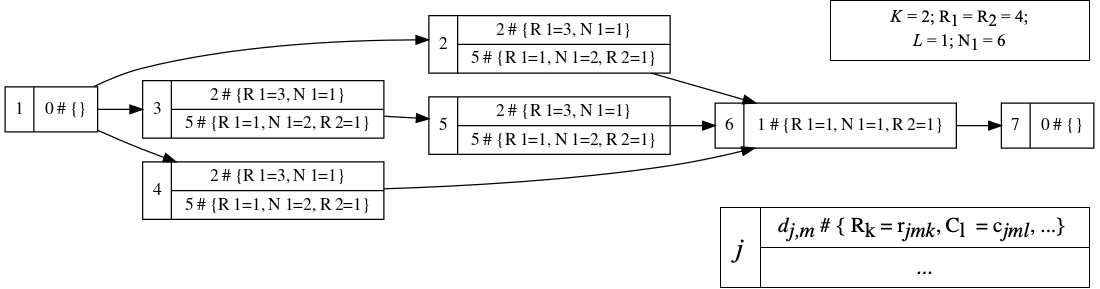
\includegraphics[width=1.1\textwidth]{assets/img/02_Grundlagen/ExampleProjectMRCPSP_Plan.png}
    }
    \caption{Graphen-Darstellung eines \ac{mrcpsp} Beispiel-Projektplans mit $|J| = 7$ Aktivitäten} 
    \label{img:example_mrcpsp}
    \source{Eigene Darstellung}
\end{figure}

Abbildung \ref{img:example_mrcpsp} zeigt eine grafische Darstellung eines \ac{mrcpsp} Beispielprojektes mit 7 Aktivitäten dar, wobei $J_0$ und $J_7$ die Dummy-Knoten entsprechen. Innerhalb der Aktivitätsknoten befinden sich zudem die zugehörigen ausführbaren Modi mit deren Zeit- und Ressourcenanforderungen. Die Aktivitäten $J_2 \, ... \, J_4$ können jeweils in zwei verschiedenen Versionen ausgeführt werden, sofern die Beschränkungen eingehalten werden. \\

\begin{figure}[H]
    \centering
    \noindent\makebox[\textwidth]{%
    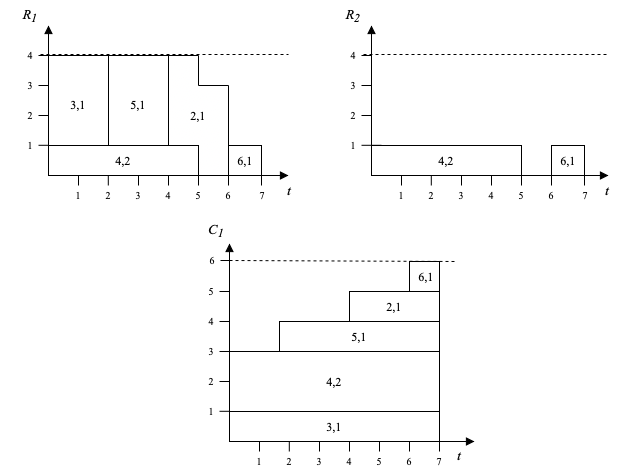
\includegraphics[width=1.1\textwidth]{assets/img/02_Grundlagen/ExampleProjectMRCPSP_Schedule.png}
    }
    \caption{Möglicher Zeitplan zum \ac{mrcpsp} Beispiel-Projektplan} 
    \label{img:example_mrcpsp_schedule}
    \source{Eigene Darstellung}
\end{figure}

Abbildung \ref{img:example_mrcpsp_schedule} zeigt für den \ac{mrcpsp} Beispiel-Projektplan eine optimale Belegung aller Ressourcenarten auf. In der Grafik wurden für alle Aktivitäten auch die zugehörigen Modi gekennzeichnet. Der Makespan für diesen (optimalen) Zeitplan liegt bei $C_{max} = 7$. Dadurch, dass sich nicht-erneuerbare Ressourcen $C_l$ nicht regenerieren, wird dieses Verhalten bei der Ressourcenbelegungsabbildung dahingehend berücksichtigt, dass jede gestartete Aktivität bis zum Projektende andauert. Es lässt sich erkennen, dass für das Beispiel am Projektende keine nicht-erneuerbaren Ressourcen mehr zur Verfügung stehen und folglich das Ausführen von weiteren Aktivitäten über den zweiten Modus zu invaliden Schedules führen würde. Der Verbrauch von nicht-erneuerbaren Ressourcen wäre im zweiten Modus bei allen Aktivitäten im Beispiel-Projektplan höher als bei dem ersten Modus und folglich würde die Grenze $C_l$ überschritten werden. \\
Aufgrund der nicht-erneuerbaren Ressourcenanforderungen und der Möglichkeit, Aktivitäten über verschiedene Modis auszuführen bewies \cite[S. 3 f.]{kolisch_local_1997}, dass sich das \ac{mrcpsp} nicht um ein $\mathcal{NP}$-hartes, sondern sogar um ein $\mathcal{NP}$-vollständiges Problem handelt. Dies ist dann der Fall, wenn mehr als zwei nicht-erneuerbare Ressourcenarten $|L| \geq 2$ und nicht-Dummy Aktivitäten in mehr als zwei Modi $\exists j \in J \, / \, \{ J_0, J_{j+1} \}: |M_j| \geq 2$ ausgeführt werden können \cite[vgl.][S. 3 f.]{kolisch_local_1997}. Durch die Auswahl der Modi wird direkt der Verbrauch an nicht-erneuerbaren Ressourcen beeinflusst. Die nicht-erneuerbaren Ressourcenanforderungen können nach Selektion der Modi die verfügbare Kapazität $C_l$ überschreiten, was ein Schedule gemäß Bedingung \ref{align:mrcpsp_constraint4} ungültig macht. \\

Heuristiken basierend auf prioritätsbasierten Regeln stellen für die Berechnung von Schedules auch beim \ac{mrcpsp} eine wichtige Technik für das Finden von adäquaten, wenn aber nicht optimalen Lösungen dar. Diese werden im Abschnitt \ref{subsec:SGS} genauer beleuchtet. Bei komplexen Projekten mit mehr als 20 Aktivitäten kommen Heuristiken an ihre Grenzen. Folglich werden Metaheuristiken eingesetzt, welche mittels lokaler Suche versuchen die optimale Lösung zu finden. Viele Metaheuristiken benötigen initiale Lösungen, wofür Heuristiken jedoch eine gute Basis darstellen. \cite[vgl.][S. 69 f.]{lova_multi-mode_2006} 